% Created by tikzDevice version 0.10.1 on 2016-08-26 08:50:02
% !TEX encoding = UTF-8 Unicode
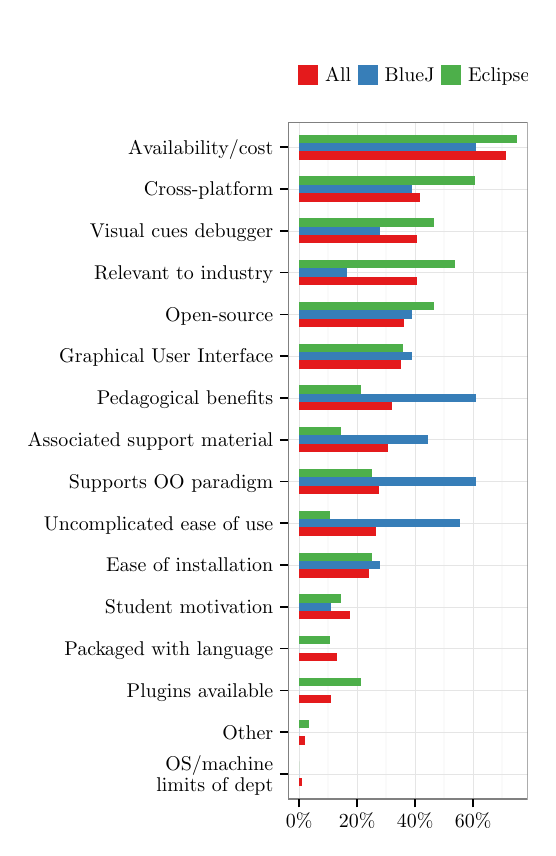
\begin{tikzpicture}[x=1pt,y=1pt]
\definecolor{fillColor}{RGB}{255,255,255}
\path[use as bounding box,fill=fillColor,fill opacity=0.00] (0,0) rectangle (180.67,289.08);
\begin{scope}
\path[clip] (  0.00,  0.00) rectangle (180.67,289.08);
\definecolor{drawColor}{RGB}{255,255,255}
\definecolor{fillColor}{RGB}{255,255,255}

\path[draw=drawColor,line width= 0.6pt,line join=round,line cap=round,fill=fillColor] (  0.00,  0.00) rectangle (180.68,289.08);
\end{scope}
\begin{scope}
\path[clip] ( 94.14, 10.36) rectangle (180.67,254.94);
\definecolor{fillColor}{RGB}{255,255,255}

\path[fill=fillColor] ( 94.14, 10.36) rectangle (180.67,254.94);
\definecolor{drawColor}{gray}{0.98}

\path[draw=drawColor,line width= 0.6pt,line join=round] (108.56, 10.36) --
	(108.56,254.94);

\path[draw=drawColor,line width= 0.6pt,line join=round] (129.54, 10.36) --
	(129.54,254.94);

\path[draw=drawColor,line width= 0.6pt,line join=round] (150.52, 10.36) --
	(150.52,254.94);

\path[draw=drawColor,line width= 0.6pt,line join=round] (171.50, 10.36) --
	(171.50,254.94);
\definecolor{drawColor}{gray}{0.90}

\path[draw=drawColor,line width= 0.2pt,line join=round] ( 94.14, 19.42) --
	(180.67, 19.42);

\path[draw=drawColor,line width= 0.2pt,line join=round] ( 94.14, 34.51) --
	(180.67, 34.51);

\path[draw=drawColor,line width= 0.2pt,line join=round] ( 94.14, 49.61) --
	(180.67, 49.61);

\path[draw=drawColor,line width= 0.2pt,line join=round] ( 94.14, 64.71) --
	(180.67, 64.71);

\path[draw=drawColor,line width= 0.2pt,line join=round] ( 94.14, 79.81) --
	(180.67, 79.81);

\path[draw=drawColor,line width= 0.2pt,line join=round] ( 94.14, 94.90) --
	(180.67, 94.90);

\path[draw=drawColor,line width= 0.2pt,line join=round] ( 94.14,110.00) --
	(180.67,110.00);

\path[draw=drawColor,line width= 0.2pt,line join=round] ( 94.14,125.10) --
	(180.67,125.10);

\path[draw=drawColor,line width= 0.2pt,line join=round] ( 94.14,140.20) --
	(180.67,140.20);

\path[draw=drawColor,line width= 0.2pt,line join=round] ( 94.14,155.29) --
	(180.67,155.29);

\path[draw=drawColor,line width= 0.2pt,line join=round] ( 94.14,170.39) --
	(180.67,170.39);

\path[draw=drawColor,line width= 0.2pt,line join=round] ( 94.14,185.49) --
	(180.67,185.49);

\path[draw=drawColor,line width= 0.2pt,line join=round] ( 94.14,200.59) --
	(180.67,200.59);

\path[draw=drawColor,line width= 0.2pt,line join=round] ( 94.14,215.68) --
	(180.67,215.68);

\path[draw=drawColor,line width= 0.2pt,line join=round] ( 94.14,230.78) --
	(180.67,230.78);

\path[draw=drawColor,line width= 0.2pt,line join=round] ( 94.14,245.88) --
	(180.67,245.88);

\path[draw=drawColor,line width= 0.2pt,line join=round] ( 98.07, 10.36) --
	( 98.07,254.94);

\path[draw=drawColor,line width= 0.2pt,line join=round] (119.05, 10.36) --
	(119.05,254.94);

\path[draw=drawColor,line width= 0.2pt,line join=round] (140.03, 10.36) --
	(140.03,254.94);

\path[draw=drawColor,line width= 0.2pt,line join=round] (161.01, 10.36) --
	(161.01,254.94);
\definecolor{fillColor}{RGB}{228,26,28}

\path[fill=fillColor] ( 98.07, 14.89) rectangle ( 99.23, 17.91);
\definecolor{fillColor}{RGB}{77,175,74}

\path[fill=fillColor] ( 98.07, 20.93) rectangle ( 98.07, 23.95);
\definecolor{fillColor}{RGB}{55,126,184}

\path[fill=fillColor] ( 98.07, 17.91) rectangle ( 98.07, 20.93);
\definecolor{fillColor}{RGB}{228,26,28}

\path[fill=fillColor] ( 98.07, 29.99) rectangle (100.38, 33.00);
\definecolor{fillColor}{RGB}{77,175,74}

\path[fill=fillColor] ( 98.07, 36.02) rectangle (101.82, 39.04);
\definecolor{fillColor}{RGB}{55,126,184}

\path[fill=fillColor] ( 98.07, 33.00) rectangle ( 98.07, 36.02);
\definecolor{fillColor}{RGB}{228,26,28}

\path[fill=fillColor] ( 98.07, 45.08) rectangle (109.60, 48.10);
\definecolor{fillColor}{RGB}{77,175,74}

\path[fill=fillColor] ( 98.07, 51.12) rectangle (120.55, 54.14);
\definecolor{fillColor}{RGB}{55,126,184}

\path[fill=fillColor] ( 98.07, 48.10) rectangle ( 98.07, 51.12);
\definecolor{fillColor}{RGB}{228,26,28}

\path[fill=fillColor] ( 98.07, 60.18) rectangle (111.91, 63.20);
\definecolor{fillColor}{RGB}{77,175,74}

\path[fill=fillColor] ( 98.07, 66.22) rectangle (109.31, 69.24);
\definecolor{fillColor}{RGB}{55,126,184}

\path[fill=fillColor] ( 98.07, 63.20) rectangle ( 98.07, 66.22);
\definecolor{fillColor}{RGB}{228,26,28}

\path[fill=fillColor] ( 98.07, 75.28) rectangle (116.51, 78.30);
\definecolor{fillColor}{RGB}{77,175,74}

\path[fill=fillColor] ( 98.07, 81.32) rectangle (113.06, 84.34);
\definecolor{fillColor}{RGB}{55,126,184}

\path[fill=fillColor] ( 98.07, 78.30) rectangle (109.73, 81.32);
\definecolor{fillColor}{RGB}{228,26,28}

\path[fill=fillColor] ( 98.07, 90.38) rectangle (123.44, 93.39);
\definecolor{fillColor}{RGB}{77,175,74}

\path[fill=fillColor] ( 98.07, 96.41) rectangle (124.30, 99.43);
\definecolor{fillColor}{RGB}{55,126,184}

\path[fill=fillColor] ( 98.07, 93.39) rectangle (127.21, 96.41);
\definecolor{fillColor}{RGB}{228,26,28}

\path[fill=fillColor] ( 98.07,105.47) rectangle (125.73,108.49);
\definecolor{fillColor}{RGB}{77,175,74}

\path[fill=fillColor] ( 98.07,111.51) rectangle (109.31,114.53);
\definecolor{fillColor}{RGB}{55,126,184}

\path[fill=fillColor] ( 98.07,108.49) rectangle (156.35,111.51);
\definecolor{fillColor}{RGB}{228,26,28}

\path[fill=fillColor] ( 98.07,120.57) rectangle (126.89,123.59);
\definecolor{fillColor}{RGB}{77,175,74}

\path[fill=fillColor] ( 98.07,126.61) rectangle (124.30,129.63);
\definecolor{fillColor}{RGB}{55,126,184}

\path[fill=fillColor] ( 98.07,123.59) rectangle (162.17,126.61);
\definecolor{fillColor}{RGB}{228,26,28}

\path[fill=fillColor] ( 98.07,135.67) rectangle (130.35,138.69);
\definecolor{fillColor}{RGB}{77,175,74}

\path[fill=fillColor] ( 98.07,141.71) rectangle (113.06,144.73);
\definecolor{fillColor}{RGB}{55,126,184}

\path[fill=fillColor] ( 98.07,138.69) rectangle (144.69,141.71);
\definecolor{fillColor}{RGB}{228,26,28}

\path[fill=fillColor] ( 98.07,150.76) rectangle (131.50,153.78);
\definecolor{fillColor}{RGB}{77,175,74}

\path[fill=fillColor] ( 98.07,156.80) rectangle (120.55,159.82);
\definecolor{fillColor}{RGB}{55,126,184}

\path[fill=fillColor] ( 98.07,153.78) rectangle (162.17,156.80);
\definecolor{fillColor}{RGB}{228,26,28}

\path[fill=fillColor] ( 98.07,165.86) rectangle (134.95,168.88);
\definecolor{fillColor}{RGB}{77,175,74}

\path[fill=fillColor] ( 98.07,171.90) rectangle (135.53,174.92);
\definecolor{fillColor}{RGB}{55,126,184}

\path[fill=fillColor] ( 98.07,168.88) rectangle (138.86,171.90);
\definecolor{fillColor}{RGB}{228,26,28}

\path[fill=fillColor] ( 98.07,180.96) rectangle (136.11,183.98);
\definecolor{fillColor}{RGB}{77,175,74}

\path[fill=fillColor] ( 98.07,187.00) rectangle (146.77,190.02);
\definecolor{fillColor}{RGB}{55,126,184}

\path[fill=fillColor] ( 98.07,183.98) rectangle (138.86,187.00);
\definecolor{fillColor}{RGB}{228,26,28}

\path[fill=fillColor] ( 98.07,196.06) rectangle (140.72,199.08);
\definecolor{fillColor}{RGB}{77,175,74}

\path[fill=fillColor] ( 98.07,202.10) rectangle (154.26,205.12);
\definecolor{fillColor}{RGB}{55,126,184}

\path[fill=fillColor] ( 98.07,199.08) rectangle (115.56,202.10);
\definecolor{fillColor}{RGB}{228,26,28}

\path[fill=fillColor] ( 98.07,211.15) rectangle (140.72,214.17);
\definecolor{fillColor}{RGB}{77,175,74}

\path[fill=fillColor] ( 98.07,217.19) rectangle (146.77,220.21);
\definecolor{fillColor}{RGB}{55,126,184}

\path[fill=fillColor] ( 98.07,214.17) rectangle (127.21,217.19);
\definecolor{fillColor}{RGB}{228,26,28}

\path[fill=fillColor] ( 98.07,226.25) rectangle (141.88,229.27);
\definecolor{fillColor}{RGB}{77,175,74}

\path[fill=fillColor] ( 98.07,232.29) rectangle (161.75,235.31);
\definecolor{fillColor}{RGB}{55,126,184}

\path[fill=fillColor] ( 98.07,229.27) rectangle (138.86,232.29);
\definecolor{fillColor}{RGB}{228,26,28}

\path[fill=fillColor] ( 98.07,241.35) rectangle (173.00,244.37);
\definecolor{fillColor}{RGB}{77,175,74}

\path[fill=fillColor] ( 98.07,247.39) rectangle (176.74,250.41);
\definecolor{fillColor}{RGB}{55,126,184}

\path[fill=fillColor] ( 98.07,244.37) rectangle (162.17,247.39);
\definecolor{drawColor}{gray}{0.50}

\path[draw=drawColor,line width= 0.6pt,line join=round,line cap=round] ( 94.14, 10.36) rectangle (180.67,254.94);
\end{scope}
\begin{scope}
\path[clip] (  0.00,  0.00) rectangle (180.67,289.08);
\definecolor{drawColor}{RGB}{0,0,0}

\node[text=drawColor,anchor=base east,inner sep=0pt, outer sep=0pt, scale=  0.72] at ( 88.74, 20.83) {~OS/machine};

\node[text=drawColor,anchor=base east,inner sep=0pt, outer sep=0pt, scale=  0.72] at ( 88.74, 13.05) {limits of dept};

\node[text=drawColor,anchor=base east,inner sep=0pt, outer sep=0pt, scale=  0.72] at ( 88.74, 32.04) {Other};

\node[text=drawColor,anchor=base east,inner sep=0pt, outer sep=0pt, scale=  0.72] at ( 88.74, 47.13) {Plugins available};

\node[text=drawColor,anchor=base east,inner sep=0pt, outer sep=0pt, scale=  0.72] at ( 88.74, 62.23) {Packaged with language};

\node[text=drawColor,anchor=base east,inner sep=0pt, outer sep=0pt, scale=  0.72] at ( 88.74, 77.33) {Student motivation};

\node[text=drawColor,anchor=base east,inner sep=0pt, outer sep=0pt, scale=  0.72] at ( 88.74, 92.42) {Ease of installation};

\node[text=drawColor,anchor=base east,inner sep=0pt, outer sep=0pt, scale=  0.72] at ( 88.74,107.52) {Uncomplicated ease of use};

\node[text=drawColor,anchor=base east,inner sep=0pt, outer sep=0pt, scale=  0.72] at ( 88.74,122.62) {Supports OO paradigm};

\node[text=drawColor,anchor=base east,inner sep=0pt, outer sep=0pt, scale=  0.72] at ( 88.74,137.72) {Associated support material};

\node[text=drawColor,anchor=base east,inner sep=0pt, outer sep=0pt, scale=  0.72] at ( 88.74,152.81) {Pedagogical benefits};

\node[text=drawColor,anchor=base east,inner sep=0pt, outer sep=0pt, scale=  0.72] at ( 88.74,167.91) {Graphical User Interface};

\node[text=drawColor,anchor=base east,inner sep=0pt, outer sep=0pt, scale=  0.72] at ( 88.74,183.01) {Open-source};

\node[text=drawColor,anchor=base east,inner sep=0pt, outer sep=0pt, scale=  0.72] at ( 88.74,198.11) {Relevant to industry};

\node[text=drawColor,anchor=base east,inner sep=0pt, outer sep=0pt, scale=  0.72] at ( 88.74,213.20) {Visual cues debugger};

\node[text=drawColor,anchor=base east,inner sep=0pt, outer sep=0pt, scale=  0.72] at ( 88.74,228.30) {Cross-platform};

\node[text=drawColor,anchor=base east,inner sep=0pt, outer sep=0pt, scale=  0.72] at ( 88.74,243.40) {Availability/cost};
\end{scope}
\begin{scope}
\path[clip] (  0.00,  0.00) rectangle (180.67,289.08);
\definecolor{drawColor}{RGB}{0,0,0}

\path[draw=drawColor,line width= 0.6pt,line join=round] ( 91.14, 19.42) --
	( 94.14, 19.42);

\path[draw=drawColor,line width= 0.6pt,line join=round] ( 91.14, 34.51) --
	( 94.14, 34.51);

\path[draw=drawColor,line width= 0.6pt,line join=round] ( 91.14, 49.61) --
	( 94.14, 49.61);

\path[draw=drawColor,line width= 0.6pt,line join=round] ( 91.14, 64.71) --
	( 94.14, 64.71);

\path[draw=drawColor,line width= 0.6pt,line join=round] ( 91.14, 79.81) --
	( 94.14, 79.81);

\path[draw=drawColor,line width= 0.6pt,line join=round] ( 91.14, 94.90) --
	( 94.14, 94.90);

\path[draw=drawColor,line width= 0.6pt,line join=round] ( 91.14,110.00) --
	( 94.14,110.00);

\path[draw=drawColor,line width= 0.6pt,line join=round] ( 91.14,125.10) --
	( 94.14,125.10);

\path[draw=drawColor,line width= 0.6pt,line join=round] ( 91.14,140.20) --
	( 94.14,140.20);

\path[draw=drawColor,line width= 0.6pt,line join=round] ( 91.14,155.29) --
	( 94.14,155.29);

\path[draw=drawColor,line width= 0.6pt,line join=round] ( 91.14,170.39) --
	( 94.14,170.39);

\path[draw=drawColor,line width= 0.6pt,line join=round] ( 91.14,185.49) --
	( 94.14,185.49);

\path[draw=drawColor,line width= 0.6pt,line join=round] ( 91.14,200.59) --
	( 94.14,200.59);

\path[draw=drawColor,line width= 0.6pt,line join=round] ( 91.14,215.68) --
	( 94.14,215.68);

\path[draw=drawColor,line width= 0.6pt,line join=round] ( 91.14,230.78) --
	( 94.14,230.78);

\path[draw=drawColor,line width= 0.6pt,line join=round] ( 91.14,245.88) --
	( 94.14,245.88);
\end{scope}
\begin{scope}
\path[clip] (  0.00,  0.00) rectangle (180.67,289.08);
\definecolor{drawColor}{RGB}{0,0,0}

\path[draw=drawColor,line width= 0.6pt,line join=round] ( 98.07,  7.36) --
	( 98.07, 10.36);

\path[draw=drawColor,line width= 0.6pt,line join=round] (119.05,  7.36) --
	(119.05, 10.36);

\path[draw=drawColor,line width= 0.6pt,line join=round] (140.03,  7.36) --
	(140.03, 10.36);

\path[draw=drawColor,line width= 0.6pt,line join=round] (161.01,  7.36) --
	(161.01, 10.36);
\end{scope}
\begin{scope}
\path[clip] (  0.00,  0.00) rectangle (180.67,289.08);
\definecolor{drawColor}{RGB}{0,0,0}

\node[text=drawColor,anchor=base,inner sep=0pt, outer sep=0pt, scale=  0.72] at ( 98.07, -0.00) {0\%};

\node[text=drawColor,anchor=base,inner sep=0pt, outer sep=0pt, scale=  0.72] at (119.05, -0.00) {20\%};

\node[text=drawColor,anchor=base,inner sep=0pt, outer sep=0pt, scale=  0.72] at (140.03, -0.00) {40\%};

\node[text=drawColor,anchor=base,inner sep=0pt, outer sep=0pt, scale=  0.72] at (161.01, -0.00) {60\%};
\end{scope}
\begin{scope}
\path[clip] (  0.00,  0.00) rectangle (180.67,289.08);
\definecolor{fillColor}{RGB}{255,255,255}

\path[fill=fillColor] ( 89.25,263.47) rectangle (185.57,280.54);
\end{scope}
\begin{scope}
\path[clip] (  0.00,  0.00) rectangle (180.67,289.08);
\definecolor{fillColor}{RGB}{228,26,28}

\path[fill=fillColor] ( 97.84,268.45) rectangle (104.95,275.56);
\end{scope}
\begin{scope}
\path[clip] (  0.00,  0.00) rectangle (180.67,289.08);
\definecolor{fillColor}{RGB}{55,126,184}

\path[fill=fillColor] (119.39,268.45) rectangle (126.50,275.56);
\end{scope}
\begin{scope}
\path[clip] (  0.00,  0.00) rectangle (180.67,289.08);
\definecolor{fillColor}{RGB}{77,175,74}

\path[fill=fillColor] (149.53,268.45) rectangle (156.65,275.56);
\end{scope}
\begin{scope}
\path[clip] (  0.00,  0.00) rectangle (180.67,289.08);
\definecolor{drawColor}{RGB}{0,0,0}

\node[text=drawColor,anchor=base west,inner sep=0pt, outer sep=0pt, scale=  0.72] at (107.47,269.53) {All};
\end{scope}
\begin{scope}
\path[clip] (  0.00,  0.00) rectangle (180.67,289.08);
\definecolor{drawColor}{RGB}{0,0,0}

\node[text=drawColor,anchor=base west,inner sep=0pt, outer sep=0pt, scale=  0.72] at (129.02,269.53) {BlueJ};
\end{scope}
\begin{scope}
\path[clip] (  0.00,  0.00) rectangle (180.67,289.08);
\definecolor{drawColor}{RGB}{0,0,0}

\node[text=drawColor,anchor=base west,inner sep=0pt, outer sep=0pt, scale=  0.72] at (159.16,269.53) {Eclipse};
\end{scope}
\end{tikzpicture}
